%% LyX 2.1.4 created this file.  For more info, see http://www.lyx.org/.
%% Do not edit unless you really know what you are doing.
\documentclass[a4paper,ngerman,naustrian,DIV=12,BCOR=1cm]{scrbook}
\usepackage[T1]{fontenc}
\usepackage[utf8]{inputenc}
\usepackage{fancyhdr}
\pagestyle{fancy}
\setcounter{secnumdepth}{3}
\usepackage{babel}
\usepackage{textcomp}
\usepackage{url}
\usepackage{makeidx}
\makeindex
\usepackage{graphicx}
\PassOptionsToPackage{normalem}{ulem}
\usepackage{ulem}
\usepackage[unicode=true,
 bookmarks=true,bookmarksnumbered=false,bookmarksopen=false,
 breaklinks=true,pdfborder={0 0 0},backref=false,colorlinks=false]
 {hyperref}
\hypersetup{pdftitle={Hovering Steward},
 pdfauthor={Christina Bornberg, Katharina Joksch, Markus Kaiser, Alexander Punz, Lucas Ullrich},
 pdfsubject={Diplomarbeit},
 pdfkeywords={project,hexacopter,multicopter,drone,hovering,steward,autonomous,flying,blog,HTL,rennweg,event,cupcakes,restaurant,vienna,austria,technology,research}}

\makeatletter

%%%%%%%%%%%%%%%%%%%%%%%%%%%%%% LyX specific LaTeX commands.
\pdfpageheight\paperheight
\pdfpagewidth\paperwidth

%% Because html converters don't know tabularnewline
\providecommand{\tabularnewline}{\\}

%%%%%%%%%%%%%%%%%%%%%%%%%%%%%% Textclass specific LaTeX commands.
\newcommand{\strong}[1]{\textbf{#1}}
\newcommand{\code}[1]{\texttt{#1}}

%%%%%%%%%%%%%%%%%%%%%%%%%%%%%% User specified LaTeX commands.
%%%%%%%%%%%%
% Latex-Vorspann
\usepackage{lastpage}
\usepackage{listings}
\usepackage{blindtext}

%% geht nicht mit jeder Latex Variante, gibt aber ein schöneres Layout
\usepackage{microtype} 

%% Aufzählungen nicht so weit einrücken
\usepackage{enumitem}
%\setitemize{leftmargin=*} 

%\usepackage{caladea}
%\usepackage[T1]{fontenc}
\usepackage{lmodern}

\usepackage{xspace}

%% für pandoc
%% maximale Breite der Bilder
\usepackage{graphicx}
\setkeys{Gin}{width=0.90\linewidth,keepaspectratio}
\providecommand{\tightlist}{%
\setlength{\itemsep}{0pt}\setlength{\parskip}{0pt}}

%%für Bilder nebeneinander
\usepackage{subfigure}

%um Schusterjungen und Hurenkinder vermeiden zu können
\usepackage{needspace}

%Farbpaket
\usepackage{xcolor}

\makeatother

\usepackage{listings}
\addto\captionsnaustrian{\renewcommand{\lstlistingname}{\inputencoding{latin9}Listing}}
\addto\captionsngerman{\renewcommand{\lstlistingname}{\inputencoding{latin9}Listing}}
\renewcommand{\lstlistingname}{\inputencoding{latin9}Listing}

\begin{document}
%%%%%%
% Weitere Einstellungen siehe Latex-Vorspann

\sloppy % weniger Meldungen

\voffset5mm % etwas nach unten%%%%%%%%%%%%%%%%%%%%%%%%%%%%%%%%%%%%%%%%%%%%%%%%%%%%%%%%%%%%%%%%%%%%%%%%%%%%%%%%%%
% falls man die erste Zeile der Absätze nicht einrücken will
% dann sollte man aber etwas mehr Abstand zwischen den Absätzen erlauben
% Alternative \usepackage{parskip}
%%\setlength{\parindent}{0pt}
%%\setlength{\parskip}{1.5ex plus0.5ex minus0.5ex}
% Auch Fußnoten bündig ausrichten
\deffootnote[]{1em}{1em}{\textsuperscript{\thefootnotemark\ }}
% Listen etwas wenige einrücken, erfordert enumitem
\setitemize{leftmargin=*}

%%%%%%%%%%%%%%%%%%%%%%%%%%%%%%%%%%%%%%%%%%%%%%%%%%%%%%%%%%%%%%%%%%%%%%%%%%%%%%%%%%
%  Kopf und Fußzeilen -- links und rechts verschieden 
\newcommand{\kopfseitenummer}{{\bfseries \thepage}}
\newcommand{\kopfkapl}{{\bfseries\leftmark}}
\newcommand{\kopfkapr}{{\bfseries\rightmark}}
\newcommand{\kopfbild}{
\includegraphics[width=25mm]{HTL3RLogoRGB}}
\newcommand{\kopfHTL}{Höhere Technische Bundeslehranstalt Wien 3, \\Rennweg 	Abteilung für Informationstechnologie}
\renewcommand{\chaptermark}[1]%
  {\thispagestyle{fancy}\markboth{\thechapter.\ #1}{}}%\thispagestyle{fancy}

%\lhead[\fancyplain{\kopfbild}{\kopfbild}]% li aussen
%      {\fancyplain{\kopfHTL}{\kopfHTL}}% re innen
%\rhead[\kopfHTL]% li innen
%      {\kopfbild}% re aussen

%% mit kapitelautor kann man den Autor festlegen oder auf leer setzen - steht dann in der Fußzeile.
\newcommand{\kapitelautor}{}

%%%
% Alternative: am Rand (Marginale)
%\setlength{\marginparsep}{-5mm}
%\mbox{}\marginpar{\raggedleft\hspace{0pt}Autor: Hans Huber}

%% kopf links: [linke] und {rechte} Seite
\lhead[\kopfbild]{\kopfkapl}
\rhead[\kopfkapr]{\kopfbild}
\chead{}

\lfoot[\kopfseitenummer]{\kapitelautor}
\cfoot[]{}
\rfoot[\kapitelautor]{\kopfseitenummer}
\renewcommand{\footrulewidth}{0.2pt}
\renewcommand{\headrulewidth}{0.2pt}

%%
% einfaches "siehe ..." - das Ziel muss man markieren
\newcommand{\kap}[1]{Kapitel~\ref{#1}, Seite~\pageref{#1}}
\newcommand{\siehe}[1]{siehe \kap{#1}}

%% http://ieg.ifs.tuwien.ac.at/~aigner/download/tuwien.sty
%Div. Abkürzungen (in Anlehnung an Jochen Köpper, jkthesis):
%\RequirePackage{xspace}
\newcommand{\bzw}{bzw.\@\xspace}
\newcommand{\bzgl}{bzgl.\@\xspace}
\newcommand{\ca}{ca.\@\xspace}
\newcommand{\dah}{d.\thinspace{}h.\@\xspace}
\newcommand{\Dah}{D.\thinspace{}h.\@\xspace}
\newcommand{\ds}{d.\thinspace{}s.\@\xspace}
\newcommand{\evtl}{evtl.\@\xspace}
\newcommand{\ua}{u.\thinspace{}a.\@\xspace}
\newcommand{\Ua}{U.\thinspace{}a.\@\xspace}
\newcommand{\usw}{usw.\@\xspace}
\newcommand{\va}{v.\thinspace{}a.\@\xspace}
\newcommand{\vgl}{vgl.\@\xspace}
\newcommand{\zB}{z.\thinspace{}B.\@\xspace}
\newcommand{\ZB}{Zum Beispiel\xspace} 

%%%%%Anfang Titelseite
\pagenumbering{roman}
\title{Diplomarbeit}
\begin{titlepage}
\begin{minipage}[b]{1\columnwidth}
\parbox[b]{50mm}{
\includegraphics[width=45mm]{HTL3RLogoRGB}}
\hfill
\parbox[b]{130mm}{\footnotesize \textsc{Höhere Technische Bundeslehranstalt} Wien 3, Rennweg\\
IT \& Mechatronik\\
\\
HTL Rennweg :: Rennweg 89b\\
A-1030 Wien :: Tel +43 1 24215-10 :: Fax DW 18
}\\
\mbox{}
\end{minipage}

\vspace{1cm}


\begin{center}
\textbf{\LARGE{}Diplomarbeit}{\large{}}\\
{\large{}\vspace{15mm}
 }\textbf{\large{}}\\
\textbf{\large{}Hovering Steward}\\
 \vspace{15mm}
 ausgeführt an der\\
 Höheren Abteilung für Informationstechnologie/Ausbildungsschwerpunkt\\
 der Höheren Technischen Lehranstalt Wien 3 Rennweg\\
 \vspace{1cm}
 im Schuljahr 2015/2016\\
 \vspace{1cm}
 durch\\
 \vspace{0.5cm}
\textbf{\large{}Christina Bornberg}\\
\textbf{\large{}Katharina Joksch}\\
\textbf{\large{}Markus Kaiser}\\
\textbf{\large{}Alexander Punz}\\
\textbf{\large{}Lucas Ullrich}\\

\par\end{center}{\large \par}

\begin{center}
\vspace{20mm}
\normalsize unter der Anleitung von\\
\vspace{0.5cm}
Mag. Andreas Fink\\
DI Herbert Fleck
\par\end{center}

\begin{center}
\vspace{5mm}
Wien, \today 
\par\end{center}

\end{titlepage}%%%%%%%%%%%%%%%%%%%%% Ende Titelseite %%%%%%%%%%%%%%%%%%%%%

\renewcommand*{\chapterpagestyle}{fancy}

%%%%%Programmlisting%%%%%%%%
% das braucht man nur einmal
\lstset{basicstyle = \ttfamily\footnotesize,
	keywordstyle = \color{blue},
	stringstyle = \color{cyan},
	commentstyle = \color{lightgray},
	numbers = left,
	numberstyle = \tiny,
	stepnumber = 2, 
	numbersep = 5pt, 
	showspaces = false, 
	frame = single,
	escapechar = $
}
%lstset{language=...} vor jedem Listing

%hier geht es los mit dem Text - auf einer rechten Seite
\pagenumbering{arabic}
\pagestyle{fancy}
\thispagestyle{fancy} 

%\renewcommand{\kapitelautor}{Autor: VN NN} immer im Unterdokument

\thispagestyle{fancy}

\chapter{Einleitung}
\renewcommand{\kapitelautor}{Autor: Markus Kaiser}

%%%%%%%%%%%%%%%%%%%%%%%%%%%%%%%%%%%%%%%%%%%%%%%%%%%%%%%%%%%%%%%%%%%%%%%%%%%%%%%
\section{Projektidee}

%%%%%%%%%%%%%%%%%%%%%%%%%%%%%%%%%%%%%%%%%%%%%%%%%%%%%%%%%%%%%%%%%%%%%%%%%%%%%%%
\section{Ausgangssituation}
  Im den folgenden Absätzen wird beschrieben, wie die Idee von Hovering Steward, dem autonom fliegenden Kellner
  entstanden ist, und womit sich die ersten Recherchen zu Begin des Projektes beschäftigt, beziehungsweise
  welche Ergebnisse diese herausgebracht haben.

  \subsection{Ideenfindung}
  Ihren Anfang fand die Idee im Projektmanagement Unterricht. Die Teams mussten ein fiktives Projekt erfinden, um auf Basis dieses
  Projektmanagementpläne zu erstellen. Es entstand "Fluorescent Bakery", eine Bäckerei, die fluoreszierende Cupcakes verkauft.
  Der technische Teil ergab sich später, bei dem Gedanken diese Idee für die Diplomarbeit weiterzuverwenden. Der Ansatz hierfür war,
  einen nicht menschlichen Kellner zu erschaffen, der mithilife künstlicher Intelligenz die Aufgaben einer Bedienung in einem Restaurant übernimmt.
  Einen Kellner auf Rädern erschien zu simpel, daher wurde die Entscheidung getroffen, die 3. Dimension mit einzubeziehen und ihn fliegen zu lassen.
  So entstand "Hovering Steward - der autonom fliegende Kellner", ein dreidimensionales Tracking-System, welches eine Drohne in einem Raum die Aufgaben eines Kellners durchführen lässt.
  Das Projekt erhielt später noch eine weitere Komponente, nämlich eine digitale Speisekarte, um das System in einem Restaurant vollständig zu automatisieren.

  \subsection{Was es schon gibt}

  \textbf{Themenrestaurants}
  \begin{itemize}
    \item Disaster Café\\
    Das Themenrestaurant Disaster Café in Spanien bietet Gästen die Erfahrung, ihr Essen bei einem Erdbeben
    der Stärke 7.8 zu sich zu nehmen.

    \item Das stille Örtchen - Modern Toilet\\
    Eingerichtet wie eine Toilette, können Gäste des Modern Toilet in Japan ihre Speisen in einem gewohnten Umfeld genießen.

    \item Affen-Kellner\\
    Die kleine Taverne in Japan besitzt zwei kleine Affen, die Tätigkeiten wie das Servieren von Getränken oder Handtüchern
    für den Inhaber übernehmen. Sie verstehen sogar, welche Getränke ein Gast bestellt.

    \item The Royal Dragon\\
    Neben Rollschuh fahrenden Kellnern verfügt das weltweit größte Restaurant für Meeresfrüchte eine
    Art Seilbahn, mithilfe welcher ein Kellner "fliegend" das Essen serviert.

    \item Dinner in the Sky\\
    Bei Dinner in the Sky werden dee Gäste samt Tisch und kleiner Küche von einem Kran 50 Meter
    in die Luft gezogen, wo dann gespeist wird.

    \item Dinner in the Dark\\
    In diesem Themenrestaurant verbringen die Gäste ihren Aufenthalt im Dunkeln. Einzig und allein die
    Kellner können mittels Nachtsichtbrille etwas sehen.
  \end{itemize}

  \textbf{Multicopter in der Gastronomie}
  \begin{itemize}
      \item{Infinium-Serve}\\
      Das Unternehmen Infinium-Robotics hat ein System entwickelt, welches Gästen eines Restaurants
      das Essen mittels Hexacopter serviert.

      \item{iTray}\\
      iTray, ein Projekt aus London, nutzt kleine Drohnen um Sushi an die Tische der Gäste zu bringen.
      Die Drohnen werden über ein Remote-Wi-Fi-System gesteuert.

  \end{itemize}

%%%%%%%%%%%%%%%%%%%%%%%%%%%%%%%%%%%%%%%%%%%%%%%%%%%%%%%%%%%%%%%%%%%%%%%%%%%%%%%
\section{Team und Aufgabenverteilung}
  \textbf{Markus Kaiser}\\
  \textbf{Projektleitung und Marketing}\\
  Markus Kaiser leitete das Team Hovering Steward und war somit für das Projektmanagement und
  die organisatorischen Aspekte verantwortlich. Neben dieser Hauptrolle zählte außerdem das Marketing
  zu seinen Aufgabenbereichen, was speziell die Entwicklung des Blogs anbelangte. Durch seine Kenntnisse
  in der Webentwicklung stellte er mit dem Blog eine wichtige Schnittstelle zur Außenwelt her.

  \textbf{Lucas Ullrich}\\
  \textbf{Sensorik & Firmware}\\
  Lucas Ullrich war neben seiner Position als Projektleiter Stellvertreter für die Sensorik an unserer Drohne und
  für die Programmierung der Firmware zuständig. Er unterstützte unseren Projektleiter bei terminlichen Angelegenheiten
  und konnte durch seine Kenntnisse mit der Programmiersprache C eine solide Basis für die Firmware des Microcontrollers schaffen.
  Außerdem

  \textbf{Christina Bornberg}\\
  \textbf{Firmware}\\
  Christina Bornberg fungierte als Firmware Entwicklerin des Teams. Durch ihre Interesse an der Programmierung von Drohnen
  und bereits gesammelten Erfahrung mit der Programmierung von C konnte sie gemeinsam mit Lucas Ullrich die LOgik hinter
  dem automatisierten Flug der Drohne realisieren.

  \textbf{Katharina Joksch}\\
  \textbf{Webentwicklung}\\
  Der Aufgabenbereich von Katharina Joksch war die Webentwicklung, genauer gesagt die Programmierung der digitalen Speisekarte.
  Neben der Planung der Datenbank und der sinnvollen Verwendung hilfreicher Frameworks entwickelte sie außerdem eine Java Applikation,
  die die Kommunikation zwischen der Speisekarte und der Drohne regelte.

  \textbf{Alexander Punz}\\
  \textbf{Hardware & Mechanik}\\
  Alexander Punz war sowohl für die Hardware als auch für die Mechanik verantwortlich. Seine Aufgaben waren sowohl die Konzeption
  und Produktion des Rotorschutzes, der einen sicheren Flug der Drohne ermöglichte, als auch die Herstellung diverser Halterungen,
  die für Sensorik, Transport und Flugtests verausgesetzt waren.

%%%%%%%%%%%%%%%%%%%%%%%%%%%%%%%%%%%%%%%%%%%%%%%%%%%%%%%%%%%%%%%%%%%%%%%%%%%%%%%
\section{Betreuer}
  \textbf{Mag. Andreas Fink}\\
  Mag. Andreas Fink stand dem Projektteam als Hauptbetreuer der Abteilung für Informationstechnologie zur Seite.
  Seine objektive Sichtweise auf das Projekt, hat dem Team sehr geholfen den Fokus auf die Ziele zu legen und
  das Projekt in die Richtung zu entwickeln.
  Zusätzlich dazu betreute er individuell Markus Kaiser bei den Aspekten Projektleitung und Marketing.

  \textbf{DI Herbert Fleck}\\
  DI Herbert Fleck war Hauptbetreuer der Mechatronik Abteilung unseres Teams. Er koordinierte den Prozess der Diplomarbeit
  gemeinsam mit Mag. Andreas Fink. Das Teeam schätzte außerdem sehr das Konstruktive Feedback bei Präsentationen.
  Er betreute nebenbei Lucas Ullrich mit Fachwissen aus dem Bereich der Elektronik.

  \textbf{DI August Hörandl}\\
  DI August Hörandl fungierte als Individualbetreuer von Christina Bornberg. Duch seine Fähigkeiten und
  Erfahungen als Programmierer sowohl mit der Sprache C, als auch Java war das Entwickeln der Firmware,
  aber auch der Java-Applikation für die WLAN-Kommunikation wesentlich einfacher. Außerdem war
  DI August Hörandl unser Ansprechpartner wenn es Unklarheiten bei LaTeX gab.

  \textbf{MMag. Florian Weiss}\\
  MMag. Florian Weiss betreute Katharina Joksch bei der Entwicklung der digitalen Speisekarte. Sein umfangreiches
  Know-How im Bereich der Webentwicklung, dem Umgang mit diversen Frameworks und Bibliotheken half Katharina
  dabei ein Grundgerüst für die Entwicklung aufzubauen.

  \textbf{DI Franz Temper}\\
  DI Franz Temper unterstützte Alexander Punz bei der Enticklung der Konstuktionen.

%%%%%%%%%%%%%%%%%%%%%%%%%%%%%%%%%%%%%%%%%%%%%%%%%%%%%%%%%%%%%%%%%%%%%%%%%%%%%%%
\section{Partner / Sponsoren}


%%%%%%%%%%%%%%%%%%%%%%%%%%%%%%%%%%%%%%%%%%%%%%%%%%%%%%%%%%%%%%%%%%%%%%%%%%%%%%%
\section{Danksagung}

\chapter{Projektmanagement}
\renewcommand{\kapitelautor}{Autor: Markus Kaiser}

%%%%%%%%%%%%%%%%%%%%%%%%%%%%%%%%%%%%%%%%%%%%%%%%%%%%%%%%%%%%%%%%%%%%%%%%%%%%%%%
\section{Ziele}

  \subsection{Muss-Ziele}
  \textbf{RE-M 01 Blog}\\
  Die Diplomarbeitswebsite fungiert in erster Linie als selbst programmierter Blog, um Interessenten
  jederzeit die Möglichkeit zu bieten, sich über den Status des Projektes zu informieren. Jedes Teammitglied
  kann individuelle Blog- oder Entwicklertagebucheinträge verfassen.

  \textbf{RE-M 02 Facebookauftritt}\\
  Eine Facebookseite names "Hovering Steward" ist erstellt. Sie informiert Interessenten über das
  Projekt und den Blog. Sponsoren sind genannt und das Diplomarbeitsteam ist vorgestellt.

  \textbf{RE-M 03 Sponsoren und Finanzen}\\
  Um die Kosten des Projektes zu decken, sind diverse Unternehmen, die möglicherweise Interesse an dem
  Projekt haben, per e-Mail oder telefonisch kontaktiert, und um eine Partnerschaft gefragt worden.
  Für kooperative Firmen sind diverse webetechnische Gegenmaßnahmen geplant worden, um das Sponsoring
  zu decken.

  \textbf{RE-M 04 Abrufbarkeit auf Tablets}\\
  Die digitale Speisekarte steht für Gäste auf Tablets zur Verfügung. Damit der Gast bestellen kann,
  ruft der User die Anwendung auf. Das Tablet benötigt zum Abruf der App mindestens einen der Browser
  Safari 7, Firefox 30 oder Internet Explorer 11.

  \textbf{RE-M 05 Speiseinformationen}\\
  Damit die Speisekarte der anerkannten Norm entspricht, enthält sie Informationen über die Inhaltsstoffe
  beziehungsweise Allergikerinformationen. Auf dem Screen der Speiseinformationen befindet sich ein
  Bestellbutton.

  \textbf{RE-M 06 Datenverwaltung}\\
  Die Daten der Speisekarte ruft die Webapp über eine Datenbank ab. Die Schnittstellen stehen für eine
  HTML und JSON Ausgabe zur Verfügung.

  \textbf{RE-M 07 Bestellfunktion}\\
  Durch den Klick auf den "Bestellbutton", der sich auf dem Speiseinformationsscreen befindet, wird eine
  Speise bestellt. Die Bestellung erscheint im Adminbereich der Applikation, auf einem anderen Gerät mit mindestens einem der Betriebssysteme
  OS X Yosemite oder Windows 8, und auf dem zusätzlich mindestens einer der Browser Safari 7, Firefox 30,
  Google Chrome oder Internet Explorer 11 installiert ist.

  \textbf{RE-M 08 Adminbereich}\\
  Nachdem eine Speise bestellt worden ist, erscheint ein neuer Bestelleintrag mit Bezeichnung der Speise
  und Tischinformation in einer Liste auf einem PC oder Laptop.

  \textbf{RE-M 09 Responsive Layout}\\
  Das Layout der Speisekarte passt sich automatisch an die Größe des Geräts, von welchem es aufgerufen wird, an.

  \textbf{RE-M 10 Testen der Konzeptstudien}\\
  Um festzustellen ob sich die erarbeiteten Konzepte auch in der Praxis bewähren und somit einen Einsatz zu
  teuren Kameratrackingsystemen schaffen zu können, sind diese umgesetzt. Als Sensoren sind eine Kamera
  sowie Ultraschallsensoren verwendet. Um weitere Positionen zu markieren arbeitet der Multicopter mit
  Farbcodes und/oder Infrarotsendern.

  \textbf{RE-M 11 Konzeptstudie: Sensorik}\\
  Um ohne manuelle Einfüsse fliegen zu können und sein Ziel zu finden braucht der Multicopter eine Reihe
  von Sensoren. Diese dienen zur Positions-bzw. zur Objekterfassung.

  \textbf{RE-M 12 Konzeptstudie: Tischplan}\\
  Um eine vorgegebene Route fliegen zu können muss der Multicopter einen Routenpan vorgegeben bekommen.
  In diesem sind die einzelnen Markierungspunkte enthalten, welche der Multicopter auf seinem Weg zum
  Tisch überfliegt.

  \textbf{RE-M 13 Konzeptstudie: Navigation}\\
  Um zu dem richtigen Tisch zu kommen, muss der Multicopter anhand des Tischplans zu diesem
  navigieren. Im Tischplan sind die Routen und Tischpositionen hinterlegt.

  \textbf{RE-M 14 Konzeptstudie: Kommunikation}\\
  Ein Konzept zur Kommunikation zwischen Multicopter und Sensoren ist entworfen.
  Der Multicopter ist mit den Sensoren verbunden. Von diesen bekommt er die nötigen Informationen.

  \textbf{RE-M 15 Konzeptstudie: Positionserkennung}\\
  Um durch den Raum navigieren zu können muss der Multicopter Informationen zu seiner Position haben.
  Diese kann er anhand einiger Sensoren selbst auswerten und weiterverarbeiten.

  \textbf{RE-M 16 Konzeptstudie: Objekterkennung}\\
  Der Multicopter soll während seinem Flug bestimmte Objekte erkennen können, so z.B. Tische,
  Personen oder Landeplattformen.

  \textbf{RE-M 17 Konzeptstudie: Systemausfall-Maßnahmen}\\
  Tritt bei dem Multicopter ein Systemausfall ein, landet das Flugobjekt und gibt eine Fehlermeldung aus.
  Weiters besteht die Möglichkeit, in den manuellen Flugmodus umzusteigen.

  \textbf{RE-M 18 Konzeptstudie: Sicherheitsmaßnahmen (Software)}\\
  Bei Erkennung eines Hindernisses, welches eine Gefahr für den Multicopter darstellt muss dieser
  entsprechend reagieren. Stationären Objekten wie zum Beispiel Wänden weicht er, sofern dies
  möglich ist, aus. Erkennt er Personen in unmittelbarer Nähe landet er.

  \textbf{RE-M 19 Zusammenbau des Multicopters}\\
  Der ausgewählte Multicopter ist soweit zusammengebaut, dass er flugfähig ist.

  \textbf{RE-M 20 Auswahl der Bauteil (Multicopter)}\\
  Um einen flugfähigen Multicopter zu schaffen, bedarf es mehrerer Bauteile, diese sind ausgewählt
  und bestellt. Dazu zählen unter anderem: Fernbedienung, Gestell, Motoren, Rotorblätter,
  FlightController, Akkus.

  \textbf{RE-M 21 Auswahl der Bauteile (Elektronik)}\\
  Die Sensoren für einen autonomen Flug des Multicopters sind anhand des Sensorkonzepts
  ausgewählt. Weiters ist ein Mikrocontroller ausgewählt, der die Steuerung des Multicopters
  übernimmt.

  \textbf{RE-M 22 Blog Team Nutzerkontos}\\
  Für jedes Teammitglied ist ein Benutzerkonto angelegt, damit individuell Blogeinträge
  verfasst werden können. Zusätzlich zu Namen, kann ein Benutzername, eine e-Mail Adresse
  als Kontaktmöglichkeit und eine "Lieblingsfarbe" angegeben werden.

  \textbf{RE-M 23 Blog Login}\\
  Jedes Teammitglied kann sich mit dem individuell angelegten Benutzerkonto anmelden,
  um Blogeinträge zu verfassen. Nur angemeldeten Benutzern ist es möglich Blogeinträge zu
  verfassen.

  \textbf{RE-M 24 Blog Responsive Design}\\
  Bei Verwendung von kleinen Geräten, wie Smartphones oder Tablets verändert sich die
  Anordnung und Darstellung einzelner Elemente so, dass eine gute Usability auch bei mobilder
  Nutzung des Blogs gewährleistet ist.

  \subsection{Optionale Ziele}
  \textbf{RE-O 01 Speisen verwalten}\\
  Der Adminscreen beinhaltet die Funktion Speisen hinzuzufügen und zu löschen.

  \textbf{RE-O 02 Kategorien}\\
  Bevor der Gast auf den Screen mit den einzelnen Speisen verwiesen worden ist, muss er
  eine Kategorie auswählen, in der die dazugehörigen Speisen gesammelt sind. Anschließend
  sind die Speisen, welche in die ausgewählte Kategorie gehören, aufgelistet.

  \textbf{RE-O 03 Farbcodes für Tische}\\
  Der Admin hat die Möglichkeit den Tischnummern Farbcodes zuzuteilen. Anhand der
  Farbcodes findet der Multicopter die einzelnen Tische.

  \textbf{RE-O 04 Platinenanfertigung}\\
  Die Platinen für die Kommunikation zwischen dem Multicopter, der
  Basis und den Zwischenstationen werden angefertigt und bestückt.

  \textbf{RE-O 05 Sensorik (Hardware)}\\
  Das Positionierungssystem erfordert Sensoren, damit der Multicopter weiß, wo er
  ist, beziehungsweise wo er landen soll. Diese Sensoren sind an dem Multicopter
  mittels Halterungen befestigt.

  \textbf{RE-O 06 Objekttransport - Einfache Transportplatte}\\
  Die Haltevorrichtung ist an dem Multicopter montiert, um ein Objekt transportieren zu können.
  Das Objekt wird auf dem Multicopter platziert und bis zu dem Gast transportiert.
  Die Haltevorrichtung ist möglichst einfach aufgebaut, um Gewicht zu sparen.

  \textbf{RE-O 07 System aufsetzen}\\
  Die einzelnen Komponenten des Multicopters sind miteinander verbunden und er ist
  durch eine manuelle Steuerung flugfähig. Die Entwicklungsumgebung für die
  Programmierung der Software und somit der automatischen Steuerung ist installiert.

  \textbf{RE-O 08 Kommunikation}\\
  Der Multicopter ist mit den ausgewählten Sensoren verbunden. Er kann Befehle geben,
  Informationen empfangen und diese verarbeiten.

  \textbf{RE-O 09 Auswertung Serverdaten}\\
  Der Multicopter empfängt die Tischinformation über Bluetooth/WLAN vom Server,
  wertet diese aus und verarbeitet sie im Anschluss.

  \textbf{RE-O 10 Grundfunktion Multicopter: Starten}\\
  Steigen/Starten, wird durch höhere Drehzahlen erreicht.

  \textbf{RE-O 11 Grundfunktion Multicopter: Landen}\\
  Negative Steigung/Landen, wird durch niedrigere Drehzahlen erreicht.

  \textbf{RE-O 12 Grundfunktion Multicopter: Rollen}\\
  Wenn sich die rechten Propeller schneller als die linken drehen, neigt sichder
  Multicopter nach links und fliegt in diese Richtung. Wenn sich die linken Propeller
  schneller drehen, fliegt er nach rechts.

  \textbf{RE-O 13 Grundfunktion Multicopter: Nicken}\\
  Durch Neigung wird Vortrieb erzeugt. Beim Vorwärtsflug drehen sich die hinteren
  Rotoren schneller, beim Rückwärtsflug die Vorderen.

  \textbf{RE-O 14 Grundfunktion Multicopter: Gieren}\\
  Der Multicopter dreht sich um seine eigene Hochachse, wenn die Drehzahlen der
  Rotorenpaare unterschiedlich sind. Wenn sich die nach links drehenden Rotoren schneller
  bewegen, dreht er sich nach links und umgekehrt nach rechts.

  \textbf{RE-O 15 Blog Entryfilter}\\
  Nutzer des Blogs haben die Möglichkeit sich Blogeinträge nach Autor oder nach
  Art des Eintrags (Blogeintrag oder Entwicklertagebuch) sortieren zu lassen.

  \textbf{RE-O 16 Blog Benutzerkonto bearbeiten}\\
  Es gibt die Möglichkeit für die Teammitglieder Informationen wie Benutzername,
  Farbe oder E-Mail Adresse im Nachhinein zu ändern.

  \textbf{RE-O 17 Blog Statistiken}\\
  Auf dem Dashboard des Blogs sind Informationen, wie zum Beispiel die Anzahl der
  verfassten Blogs, zu sehen. Loggt sich ein Teammitglied ein, sieht es diese Werte
  noch einmal auf die eigenen Blogs bezogen.

  \textbf{RE-O 18 Datenverkehr mit Multicopter}\\
  Durch einen Klick auf den „Servierbutton“, der sich auf der Bestellliste des
  Adminscreens neben jedem Eintrag befindet, bekommt der Multicopter die Tischinformation
  des Gastes, um dessen Bestellung es sich handelt, drahtlos zugeschickt. Dies geschieht
  entweder durch eine Datenübertragung von dem Gerät auf dem der Adminbereich geöffnet
  ist an das Flugobjekt oder durch eine manuelle Eingabe der Tischinformation in eine
  bereits existierende Anwendung, welche die Daten an den Multicopter schickt.

  \subsection{Optionale Erweiterungen}

  \subsection{Nicht-Ziele}

%%%%%%%%%%%%%%%%%%%%%%%%%%%%%%%%%%%%%%%%%%%%%%%%%%%%%%%%%%%%%%%%%%%%%%%%%%%%%%%
\section{Projektmanagement-Methode}

  \subsection{Kanban}

  \subsection{Wasserfall}

  \subsection{Scrum}

%%%%%%%%%%%%%%%%%%%%%%%%%%%%%%%%%%%%%%%%%%%%%%%%%%%%%%%%%%%%%%%%%%%%%%%%%%%%%%%
\section{Teammanagement / Teambuilding}

  \subsection{KaTeCos}

  \subsection{Playground-Meetings}

  \subsection{Sonstiges}


\chapter{Elektronik}
\renewcommand{\kapitelautor}{Autor: Lucas Ullrich}

%%%%%%%%%%%%%%%%%%%%%%%%%%%%%%%%%%%%%%%%%%%%%%%%%%%%%%%%%%%%%%%%%%%%%%%%%%%%%%%
\section{Allgemeine technische Planung}

  \subsection{Benötigte Elemente}

    \subsubsection{PIC}

    \subsubsection{DJI NAZA-M lite, Flamewheel F550}

%%%%%%%%%%%%%%%%%%%%%%%%%%%%%%%%%%%%%%%%%%%%%%%%%%%%%%%%%%%%%%%%%%%%%%%%%%%%%%%
\section{Blockschaltbild}

  \subsection{Hauptplatine}

    \subsubsection{Technische Planung}

    \subsubsection{Umsetzung}

    \subsubsection{Herausfoderungen und Lösungen}

  \subsection{WLAN}

    \subsubsection{Technische Planung}

    \subsubsection{Umsetzung}

    \subsubsection{Herausfoderungen und Lösungen}


% !TEX root = diplomarbeit.tex
\chapter{Firmware}
\renewcommand{\kapitelautor}{Autor: Christina Bornberg, Lucas Ullrich}

%%%%%%%%%%%%%%%%%%%%%%%%%%%%%%%%%%%%%%%%%%%%%%%%%%%%%%%%%%%%%%%%%%%%%%%%%%%%%%%
\section{Allgemeine technische Planung}

  \subsection{Programmiersprache}
  Zum Programmieren des Mikrocontrollers wurde die Programmiersprache C verwendet.

  \subsection{Tools}

    \begin{itemize}
      \item \textbf{yEd - Graph Editor}\\
      Zum erstellen der benötigten Flussdiagramme wurde eine Desktop Anwendung namens yEd verwendet.
      \item \textbf{GitHub}\\
      Zur Versionsverwaltung des Codes wurde die digitale Ablage GitHub verwendet. Durch diese ist eine gemeinsame Programmierung möglich.
      \item \textbf{MPLAB}\\
      MPLAB ist eine Integrierte Entwicklungsumgebung von Microchip. In dieser wurde der Mikrocontroller programmiert und anschließend das C-Programm in Assembler compiliert.
      Weiters hat die Entwicklungsumgebung eine Git Funktion, wodurch die Daten ohne zusätzliches Tool vom Server herunter- beziehungsweise hinaufgeladen werden können.
    \end{itemize}


  \subsection{Positionierungssystem - evtl an anderen Ort}

    \subsubsection{Anwendung}
    Indoor Positionierungssysteme werden derzeit vor allem zum Objekterkennung, im Umweltmonitoring, über das Detektieren von Bränden in Gebäuden,
    bis hin zum Einsatz in der Logistik verwendet. Da es sehr viele unterschiedliche Anwendungsgebiete gibt, werden unterschiedliche Methoden verwendet.

    \subsubsection{Art der Positionsbestimmung}

    Ein Lokalisierungssystem kann verschiedene Arten von Informationsdaten bereitstellen. Es gibt dazu physische, symbolische, absolute und relative Modelle.

      \begin{itemize}
        \item \textbf{Physische Positionierung}\\
        Die physische Positionierung wird in Form von Koordination bestimmt, meist in 2-D oder 3-D Karten. Längen- und Breitengrade spielen dabei eine wichtige Rolle.
        \item \textbf{Symbolische Positionierung}\\
        Symbolische Positionierung wird sprachlich beschrieben, wie \zB Küche, Keller usw.
        \item \textbf{Absolute Positionierung}\\
        Die absolute Positionierung verwendet Referenzgitter und Koordinaten. Das Paradebeispiel für absolute Ortung ist die Angabe von Längen­ und Breitengrad.
        Die darauf aufsetzende Technik, die sich diese Kartographie zu Nutze macht, ist GPS.
        \item \textbf{Relative Positionierung}\\
        Die relative Positionierung verwendet legt ihre eigenen Rahmen vor, die auf Basisstationen oder definierten Punkten basieren.
        Anders als bei der absoluten Lokalisierung muss bei der relativen Positionsbestimmung die vorherige Position des Objektes bekannt sein, auf die wird dann die Position bezogen.
      \end{itemize}


    \subsubsection{Selbst- und fernortende Lokalisierungstechniken}

    Lokalisierungstechniken können weiter als selbstortend oder fernortend (engl. self­positioning/remote­positioning) klassifiziert werden.

    Fernortende Positionierungssystem: Mobile, bewegliche Sender mit stationären, unbeweglichem Empfänger. Die Messdaten aller Empfänger werden gesammelt und die
    Position des Senders wird in der Zentrale berechnet. Hier ist ein Netzwerk notwendig, sämtliche Berechnungen werden durch eine zentrale Instanz ausgeführt.

    Selbstortende Positionierungssystem: Der mobile, bewegliche Empfänger bekommt die Daten von verschiedenen Sendern, die sich auf bekannten Positionen befinden.
    Die Lokalisation des Empfängers wird durch die gemessenen Signale ermittelt. Das Objekt kann sich selbst orten, es ist kein Netzwerk notwendig.



    \subsubsection{Algorithmen}

    Prinzipiell gibt es vier Möglichkeiten, eine Positionierung vorzunehmen.
    \begin{itemize}
      \item Lateration, also die Bestimmung der Position mit Hilfe von Entfernungsmessungen
      \item Angulation, hier werden Winkelmessungen zu Hilfe genommen
      \item Szenenanalyse, bei der Umgebungsparameter erfasst und ausgewertet werden
      \item Nachbarschaft (engl. proximity) bei der physische Nähe ausgenutzt wird.
    \end{itemize}

    Die dahinterstehenden Algorithmen basieren auf den Methoden der Bestimmung von Distanzen, Winkelen, Dreiecken und Nachbarschaften.

    Können die ermittelten Informationen auch mit einer vorher bestimmten Radio-Map verglichen werden bezeichnet man dieses Verfahren auch Fingerprinting.



    \subsubsection{Funktechnik}
    % die Tabelle in rosa :b %


    \textbf{Technologien}\\
    \begin{itemize}
        \item \textbf{GPS}\\
        OUTDOOR
        \item \textbf{RFID}\\
        \item \textbf{WPS}\\
      \end{itemize}

    \subsubsection{Optisches Tracking}

    \textbf{Pixy CMUcam5}\\




  \subsection{Konzepte}
  Die verschiedenen Positionierungsarten wurden verwendet, um Konzepte für die Navigation zu entwickeln.

    \subsubsection{Aufgabenstellung}
    Damit der Hexacopter autonom durch den Raum navigieren kann, benötigt er ein Positionierungssystem.

    \subsubsection{Funkbasiertes Tracking}

      \textbf{Tracking mittels Signalstärke}\\

      % Das vom John ???

      Nachteile:
      Muss sehr präzise sein.
      Störungen durch andere elektromagnetische Wellen im selben Frequenzbereich.



      \textbf{Tracking mittels Laufzeitmessung}\\

      % Durch ein künstlich erstelltes lokales GPS


      % Fraunhofer: Mit Hilfe der Laufzeitmessung werden Objekte (Gegenstände oder Personen), welche mit kleinen Tags ausgestattet sind, geortet. Dazu werden Signale zwischen Sendern und Empfängern verschickt. Je nachdem, ob das Signal lange oder kurze Zeit benötigt, ist der Gegenstand weit entfernt oder ganz nah. Dies funktioniert, da man weiß, dass sich elektromagnetische Wellen mit Lichtgeschwindigkeit ausbreiten. Wird die Lichtgeschwindigkeit c mit der gemessenen Laufzeit multipliziert, kann die genaue Entfernung berechnet werden. Die Laufzeit kann mit unterschiedlichen Messprinzipien bestimmt werden, zum Beispiel mittels extrem kurzer UWB-Impulse (Ultrawideband) oder auch mit Hilfe von Korrelationsalgorithmen, die die Bekanntheit von Signalsequenzen nutzen.


    \subsubsection{Optisches Tracking}
    % Aufgrund der Komplexität einer signalbasierten


      \textbf{Kamerasystem im Raum}\\
      Verteilte Kameras in einem Raum tracken den Hexacopter mittels Marker. Dadurch kann die Position des Hexacopters bestimmt werden.


      \textbf{Linien}\\
      Zunächst wurde ein Konzept mit Linien erstellt. Der Hexacopter folgt einer einfarbigen Linie, bis er zu einer Kreuzung kommt, nun ist seine Aufgabe, die nächste Linie zu finden, um seinen Weg zum Ziel zu finden.

      Vorteile: Der Hexacopter kann die Linie nur schwer verlieren
      Nachteile: Das verwendete Kamerasystem ist nicht in der Lage eine Linie zu tracken.

      \textbf{Tracking mittels Infrarot}\\


      Vorteile:
      System funktioniert ebenfalls im Dunkeln.
      Nachteile:
      Jeder Tisch benötigt einen Stromanschluss.
      Die Wartung ist aufwändig.

      \textbf{Farbcode pro Wegabschnitt}\\
      Durch die Verwendung der Pixy CMUCam5 ergibt sich die Möglichkeit, Farbobjekte, die eine oder mehrere Farben haben, zu scannen.



      \textbf{Farbcodes variieren}\\
      Das gewählte System wird ebenfalls mittels 2-farbiger Codes umgesetzt.


      relative Positionierung ist ausreichend

      Vorteile:
      keine großartigen Kosten neben Copter und Server
      Rechnung am Hexacopter

      Nachteile:
      Aufwand im Restaurant



  \subsection{Tischkonzept}

  % Bild vom Ablauf %%%%%%%%%%%%%%%%%%%%%%%%%%%%%%%%


  \subsection{Flussdiagramme}
  Für einen besseren Überblick über die einzelnen Programme und deren geforderten Funktionen wurden einzelne Flussdiagramme des gesamten Prozesses erstellt.
  Diese dienen nachfolgend als Orientierung beim Programmieren der einzelnen Funktionen.

  \begin{figure}[tbh]
    \begin{centering}
      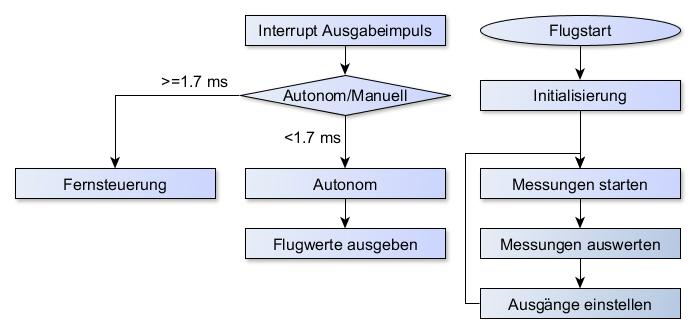
\includegraphics[width = \textwidth]{Bilder/Flussdiagramm}
    \par\end{centering}
    \caption{Flussdiagramm des Gesamtablaufs}
    \label{Flussdiragramm}
  \end{figure}

  Für die weiteren Programmteile wurden jeweils noch detailliertere Flussdiagramme erstellt.

  \subsection{Aufbau des Programms}

  % Erklärung, wer was Aufruft %





%%%%%%%%%%%%%%%%%%%%%%%%%%%%%%%%%%%%%%%%%%%%%%%%%%%%%%%%%%%%%%%%%%%%%%%%%%%%%%%
\section{Navigation}

  \subsection{Technische Planung}



    \subsubsection{Frames}

    % BILD VON LUCAS %


    \subsubsection{Aileron}
    \subsubsection{Elevator}
    \subsubsection{Rudder}

    % Rotationsbild + 2er Komplement %

    \subsubsection{Throttle}

  \subsection{Umsetzung}

    \subsubsection{Vergleichen der Frames}
    Für den Vergleich des aktuellen mit dem letzten Frame, werden zwei \glslink{Struktur}{Strukturen} verwendet, die über folgende Mitglieder verfügt.
    \begin{itemize}
      \item \textbf{num}\\
      ist die ID des getrackten Colorcodes, er besteht aus einer zweistelligen Zahl.
      \item \textbf{pos\_x}\\
      ist die X-Position des Colorcodes. Der Wert bezieht sich auf das Zentrum des Objektes.
      \item \textbf{pos\_y}\\
      ist die Y-Position des Colorcodes. Der Wert bezieht sich auf das Zentrum des Objektes.
      \item \textbf{height}\\
      ist die, vom Ultraschall übergebene Höhe.
      \item \textbf{angle}\\
      ist die Rotation des Colorcodes. Da er zweifarbig ist, kann die PIXY CMUcam5 die Rotation des Objektes feststellen.
    \end{itemize}

    Quelle: \textcolor{red}{TITEL FEHLT \cite{Structs}, das sollte verlegt werden -Lucas}

    Zuerst wird die ID des Colorcodes verglichen, um herauszufinden, ob das Farbobjekt das selbe wie im letzten Frame ist.
    Sollte dies der Fall sein, werden die Koordinaten x und y und die Rotation mit den Werten der älteren Struktur verglichen und gespeichert.
    Diese werden bei den folgenden Funktionen verwendet, um zu überprüfen, ob der Hexacopter die richtige Geschwindigkeit hat.

    \subsubsection{Aileron, Elevator und Rudder anhand der Kameradaten}
    Durch die PIXY CMUcam5 kann die Position des Hexacopters, relativ zu einem Colorcode, festgestellt werden. Gegebenenfalls werden anschließend die Flugparameter verändert.

    \begin{figure} [tbh]
      \begin{centering}
        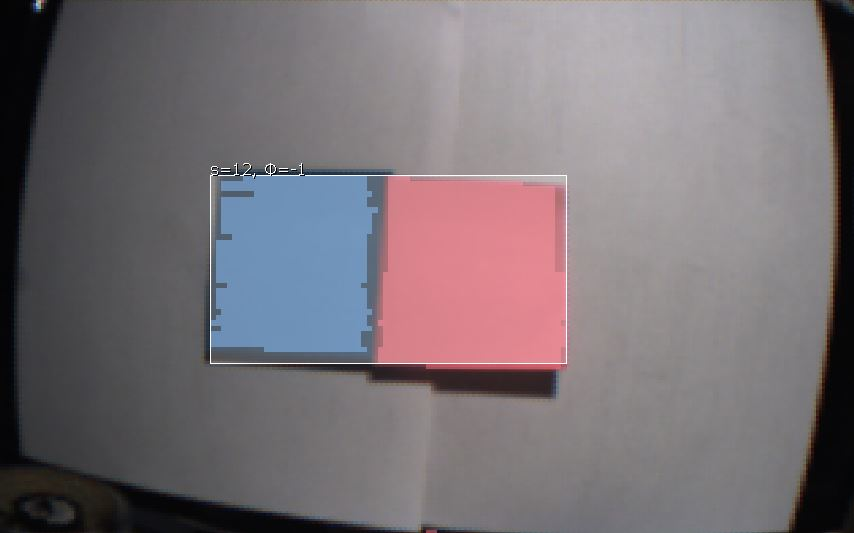
\includegraphics[width = \textwidth]{Bilder/Farbcode_erkannt}
      \par\end{centering}
      \caption{Ein erkannter Farbcode}
      \label{Farbcode_erkannt}
    \end{figure}
    Die Position wird anhand solcher Farbcodes erkannt, im Tischkonzept ist hinterlegt in welcher Reihenfolge der Hexacopter die Farbcodes suchen muss.
    Er fliegt anschließend so lange, bis er über dem aktuellen Farbcode ist, dieser also mittig im Bild ist und sucht darauf den nächsten.


    Die PIXY CMUcam5 XXXXXX % IRGENDWAS MIT X diese länge, y diese länge; %



      \begin{itemize}
        \item \textbf{Überprüfen von Aileron}\\
        Die Überprüfung von Aileron bezieht sich auf die Beschleunigung nach Links und Rechts, was der x-Koordinate entspricht.

        Ziel der Funktion ist es, den Farbcode in die Mitte des Frames zu bekommen. Der Idealzustand befindet sich zwischen 150 und 170.
        Sollte dieser Zustand erreicht werden, bleibt der Wert von Aileron unverändert und der Hexacopter fliegt weiterhin mit einer unveränderten Beschleunigung an der
        x-Koordinate.
        Sollte dies nicht der Fall sein, muss der Wert auf einige Komponenten \textcolor{red}{XXXXX} überprüft werden.
        Wenn der Farbcode zu weit auf der rechten Seite liegt, das bedeutet, wenn der Wert des Mittelpunktes vom Farbobjekt höher als 170 ist,
        muss der Hexacopter nach rechts fliegen, um seine Position zu korrigieren.
        Dabei muss zuerst verglichen werden, ob sich der Hexacopter in die richtige Richtung bewegt. Sollte er in die falsche Richtung
        fliegen, wird der Aileron-Flugparameter gesenkt, dies setzt die Beschleunigung nach Rechts vorraus.
        Wenn die Beschleunigung nach rechts hoch genug ist und die Drohne tatsächlich nach rechts fliegt, wird die Geschwindigkeit überprüft.
        Die Geschwindigkeit wird durch die Differenz der x-Koordinate beider Strukturen herausgefunden. Die Einheit ist in diesem Fall

        \item \textbf{Überprüfen von Elevator}\\
        Position der Farbobjekte (CHECK AILERON \& ELEVATOR)
        Wenn ein Farbobjekt nicht im gewünschten Bereich plaziert ist, muss der Hexacopter weiter nach links oder weiter nach rechts fliegen.
        \item \textbf{Überprüfen von Rudder}\\
        Rotation der Farbojekte (CHECK RUDDER)
        Wenn der Hexacopter über einem Farbobjekt fliegt, soll er kontrollieren, ob der 2-Farbige Code die richtige Rotation hat und sich im richtigen Bereich des Bildschirmes befindet. Wenn diese Informationen richtig sind, darf der Copter zum nächsten Farbobjekt fliegen.
        Durch dieses System könne die genauen Wege vorgegeben werden und können sich durch das gesamte Restaurant verteilen. Durch die Rotation der Codes können auch Kurven eingebaut werden.

        Richtung (CHECK RUDDER)
        Durch die Rotation der Colorcodes, kann der Hexacopter bestimmen, ob er den richtigen Weg und in die richtige Richtung fliegt, wenn er am Weg zurück zur Base ist, muss er den umgekehrten Colorcode verwenden. (Rotation 180Grad)
      \end{itemize}

    \subsubsection{Throttle anhand des Ultraschallsensors}

    Starten und landen auf Landeplattformen (CHECK THROTTLE)
    Der Hexacopter startet und landet auf den mit ebenfalls mit Colorcodes gekennzeichneten Landeplattformen.
    Bei einem Fehler, besteht auch das Landen auf einem beliebigen Fleck

    Höhe korrigieren (CHECK THROTTLE)
    Höhenunterschied zwischen Tisch und Boden

    \subsubsection{Speichern der alten Daten}

    \subsubsection{Ausgabe der Steuersignal}
    Nachdem die Steuersignale berechnet und korrigiert wurden müssen diese an den Hexacopter ausgegeben werden. Dies muss periodisch alle $\SI{20}{\milli\second}$ geschehen.
    Der Flightcontroller erkennt jeweils die einzelnen Impulse und steuert die Rotoren entsprechend an.

    Diese Impulse werden Interrupt-gesteuert ausgegeben, der Interrupt wird von dem Gear-Pin erzeugt welcher gleichzeitig für den Flugmodus verantwortlich ist.

    \lstset{language = c}
    \begin{lstlisting}
interrupt void Isr() {
  if(CCP1IF == 1) {
    CCP1IF = 0;
    T1CONbits.TMR1ON = 0;
    SignalOut();
    NOP();
  }
  if(TMR3GIF == 1) {
    TMR3GIF = 0;
    ModeCheck();
    SignalOut();    /* initial call after remaining break to 20 ms
                     * starts with Aileron (needs to be set in last
                     * case statement, case 0) following delays will
                     * be processed by the previous routine */
    pulsecounter++;
  }
}

void SignalOut(void) {
  switch(pin_out) {
    case 'A': {
      A = 1;
      Delay(a_actors[0].aile);
      pin_out = 'E';
      break;
    }case 'E': {
      A = 0;
      E = 1;
      Delay(a_actors[0].elev);
      pin_out = 'T';
      break;
    }
    \end{lstlisting}
    Die weiteren Signale (Throttle und Rudder) werden auf die gleiche Weise ausgegeben.
    Die Delay-Funktion stellt die Compare-Einehit so ein, dass nach der gewünschten Pulsdauer des Ausgangs ein Interrupt hervorgerufen wird.

%%%%%%%%%%%%%%%%%%%%%%%%%%%%%%%%%%%%%%%%%%%%%%%%%%%%%%%%%%%%%%%%%%%%%%%%%%%%%%%
\section{Objekterkennung}

  \subsection{Technische Planung}

  \subsection{Umsetzung}

  \subsection{Herausforderungen und Lösungen}

%%%%%%%%%%%%%%%%%%%%%%%%%%%%%%%%%%%%%%%%%%%%%%%%%%%%%%%%%%%%%%%%%%%%%%%%%%%%%%%
\section{Sicherheit}

  \subsection{Technische Planung}

  \subsection{Umsetzung}

  \subsection{Herausforderungen und Lösungen}

%%%%%%%%%%%%%%%%%%%%%%%%%%%%%%%%%%%%%%%%%%%%%%%%%%%%%%%%%%%%%%%%%%%%%%%%%%%%%%%
\section{Systemausfall}

  \subsection{Technische Planung}

  \subsection{Umsetzung}

  \subsection{Herausforderungen und Lösungen}


\chapter{Mechanik}

\renewcommand{\kapitelautor}{Autor: Alexander Punz}

\section{Rotorschutz}
In dem gewählten Bausatz des Hexacopters ist kein Rotorschutz beinhaltet, eines der Zeile ist es den Rotor möglichst gut zu schützen und das maximale Abfluggewicht nicht zu überschreiten. Da der Hexacopter mit einer maximalen Last von 1,9 kg belastet werden kann, können Materialen wie Stahl oder Aluminium für den Rotorschutz nicht verwendet werden. 
Da die Möglichkeit besteht, Teile in einer vernünftigen Qualität vor Ort drucken zu können, wurde die Fertigung mittels des 3D-Druckers gewählt. Mit diesem ist es möglich den erforderlichen Rotorschutz sehr genau und leicht drucken zu können. 
Die folgende Abbildung zeigt den fertigen Rotorschutz.

\begin{figure}[tbh]
\begin{centering}
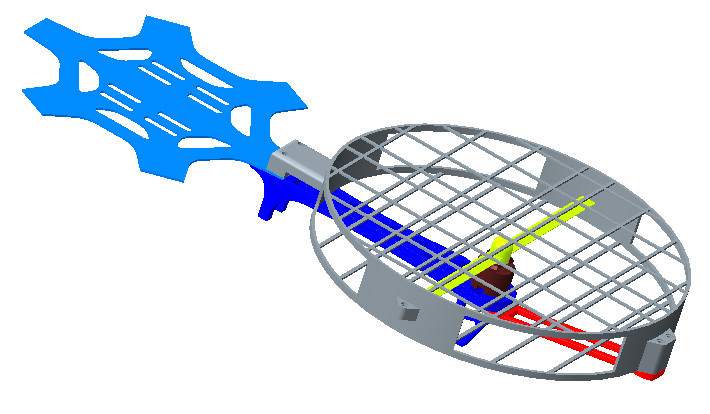
\includegraphics[width = 100mm]{Bilder/rotorschutz_zusammenbau}
\par\end{centering}
\caption{Rotorschutz systematisch dargestellt}
\label{Rotorschutz}
\end{figure}

Der Rotorschutz umrandet den Propeller, damit dieser im Falle eines Absturzes nicht zerstört wird. Die Lamellen ober- und unterhalb des Rotors sollen Personen gegen Verletzungen schützen. 
Der Ring wird durch die Strebe (rot) gestützt, damit er nicht nach unten abbrechen kann. 
Durch die großen Abmessungen bzw. der Form, kann der Ring nicht als ein Teil gedruckt werden, er wird dadurch in verschiedene Sektoren unterteilt. Der Ring wird in eine untere und obere Hälfte unterteilt bzw. beide Hälften wieder in zwei Teile. Die einzelnen Glieder werden dann mit Schrauben und Zweikomponentenkleber zusammengefügt. 

\section{Platinen}
Um das Projekt umsetzen zu können, ist es erforderlich einerseits den Mikroprozessor mit den Sensoren zu verbinden und andererseits die Kommunikation zwischen der Speisekarten-App und dem Hexacopter zu können. 
Damit diese Funktionen erfüllt werden können, werden zwei Platinen verwendet.

Das wichtigsten Bauteilgruppen der Kommunikationsplatine sind das WLAN-Modul, dieses ermöglicht die Kommunikation zwischen der App und dem Hexacopter und der Spannungsregler. Der Spannungsregler sorgt dafür, dass das WLAN-Modul mit 3.3 V versorgt wird und der Rest der Platine mit 5 V.
Die Hauptplatine beinhaltet ebenso mehrere Bereiche: Den Multiplexer, den Mikroprozessor und die Steckverbindungen für die einzelnen Sensoren.
Der Multiplexer wechslet zwischen der Steuerung der Flugmodi durch die Fernbedienung oder dem Mikroprozessor.

\begin{figure}[tbh]
\begin{centering}
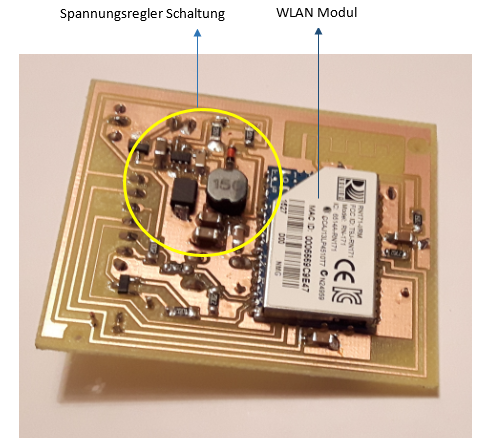
\includegraphics[width = 100mm]{Bilder/WP_Bottom_Beschriftung}
\par\end{centering}
\caption{Kommunikationsplatine Unterseite}
\label{WLAN Platine}
\end{figure}

\begin{figure}[tbh]
\begin{centering}
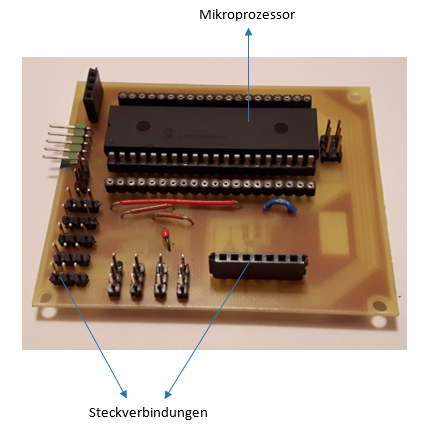
\includegraphics[width = 100mm]{Bilder/HP_Top_Beschriftung}
\par\end{centering}
\caption{Sensorplatine Oberseite}
\label{Sensor Platine oben}
\end{figure}


\begin{figure}[tbh]
\begin{centering}
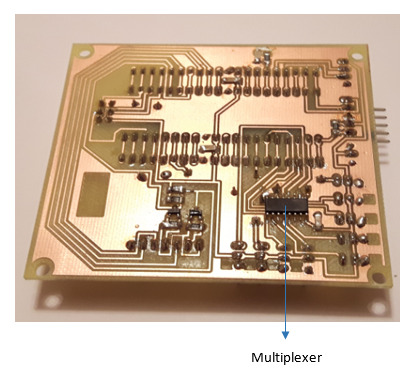
\includegraphics[width=100mm]{Bilder/HP_Bottom_Beschriftung}
\par\end{centering}
\caption{Sensorplatine Unterseite}
\label{Sensor Platine unten}
\end{figure}

\blindtext\blindtext
\chapter{Blindtext}
\blindtext

\end{document}
